\documentclass{beamer}

% Some common packages
\usepackage{graphicx, color}
\usepackage{alltt}
\usepackage{booktabs, calc, rotating}
\usepackage[round]{natbib}
\usepackage{multicol}
\usepackage{amsmath, amsbsy, amssymb, amsthm, graphicx}
\usepackage[english]{babel}
\usepackage{xkeyval} 
\usepackage{xfrac}
\usepackage[normalem]{ulem}
\usepackage{fancyvrb} 
\usepackage{tikz, geometry, tkz-graph, xcolor}
\usepackage[latin1]{inputenc}
\usepackage{times}
\usepackage[T1]{fontenc}

% Shortcuts
\newcommand{\empr}[1]{{\emph{\color{red}#1}}}
\newcommand{\cov}{\mathrm{cov}}
\newcommand{\pkg}[1]{{\textbf{\texttt{#1}}}}
\newcommand{\dif}{\mathrm{d}}
\newcommand{\bigbrk}{\vspace*{2in}}
\newcommand{\smallbrk}{\vspace*{.1in}}
\newcommand{\midbrk}{\vspace*{1in}}
\newcommand{\red}[1]{{\color{red}#1}}
\newcommand{\blue}[1]{{\color{blue}#1}}
\newcommand{\green}[1]{{\color{green}#1}}
\newcommand{\calc}[1]{{\fbox{\mbox{#1}}}}
\newcommand{\Var}{\mathrm{Var}}%
\newcommand{\Cov}{\mathrm{Cov}}%

\mode<presentation>
{
	\usetheme{UTD}
	\usecolortheme[RGB={200,0,0}]{structure}
	\setbeamercovered{transparent}
}

% fancy for Verbatim?
\fvset{frame=single,framesep=1mm,fontfamily=courier,fontsize=\scriptsize,numbers=left,framerule=.3mm,numbersep=1mm,commandchars=\\\{\}}


\title[Survival Analysis]{Applied Survival Analysis Using R\\ Chapter 4: Nonparametric Comparison of Survival Distributions}
\author[Qi Guo]{Qi Guo}
\institute[UTD]{Department of Mathematical Sciences \\ 
	The University of Texas at Dallas}
\date{April, 11 2019}
	
\begin{document}

\begin{frame}
  \titlepage
\end{frame}

% Set up UTD backgroud
\setbeamercolor*{item}{fg=red}
\bgroup
\usebackgroundtemplate{
\tikz[overlay,remember picture] \node[opacity=0.05, at=(current page.center)] {
   
\includegraphics[height=\paperheight,width=\paperwidth]{UTDbg}};}


\section[Outline]{}
\begin{frame}
  \tableofcontents
\end{frame}

\section{Comparing Two Groups of Survival Times}
\begin{frame}
\frametitle{Test Hypothesis commonly used}
\begin{itemize}
\item Typically we are interested in testing a {\color{red}null hypothesis($H_0$)} that two population {\color{red}means are equal} versus an {\color{red}alternative($H_a$)} that the {\color{red}means are not equal}(for a two-sided test)
\item  And we compute a test statistic from the {\color{red}observed} data, and \empr{reject} the null hypothesis if the test statistic \empr{exceeds} a particular constant. 
\item {\color{red}The significance level of the test($\alpha$)} is the probability that we \empr{reject} the null hypothesis when the {\color{red}null hypothesis} is in fact \empr{true}.
\item A widely known test is the {\color{red}two-sample Students t-test }for continuous observations, which requires the assumption that the observations are {\color{red}normally distributed}.
\item If the normal distribution assumption is in \empr{doubt}, a {\color{red}rank-based test} called {\color{red}the Mann-Whitney test} may be used, which gives valid test results without making parametric assumptions
\end{itemize}
\end{frame}

\pagebreak
\begin{frame}
\frametitle{Nonparametric tests of equivalence of two survival functions}
\begin{itemize}
\item {\color{red}Null Hypothesis}:\linebreak$H_0 : S_1(t) = S_0(t)$. $S_1$ and $S_0$ will represent the survival distributions for, respectively, an {\color{red}{experimental}} and a {\color{red}control therapy}.
\item {\color{red}Alternative Hypothesis}:
\begin{itemize}
\item One-sided: $H_A : S_1(t) > S_0(t)$.
\item Two-sided: $H_A : S_1(t) \neq S_0(t)$.
\end{itemize}
\item {\color{orange}$\otimes$} But it will cause the alternative can take a wide range of forms(the only equal or not is not exact enough)
\item {\color{blue}$\otimes$} What if the survival distributions are similar for some values of $t$ and differ for others?
\item {\color{purple}$\otimes$} What if the survival distributions cross?
\end{itemize}
\end{frame}

\pagebreak
\begin{frame}
\frametitle{Refine}
\begin{itemize}
\item {\color{orange}$\odot$} {\color{red}Lehman alternative}:
\begin{itemize}
\item Survival function: $S_1(t) = [S_0(t)]^{\psi}$.
\item Proportional hazard function: $h_1(t)={\psi}h_0(t)$.
\end{itemize}
\item Hence the hypothesis test will be:
\begin{itemize}
\item $H_0:\psi = 1$.
\item $H_A:\psi < 1$(subjects in Group 1 will have longer survival times than subjects in Group 0).
\end{itemize}
\item {\color{blue}$\odot$} Use rank-based test, and view the numbers of failure and numbers at risk at {\color{red}each distinct time} as a two-by-two table.
\item {\color{purple}$\odot$} Stratified Tests
\end{itemize}
\end{frame}

\pagebreak
\begin{frame}
\frametitle{Table}
For the {\color{red}$i$'th failure time} table showing: 
\begin{table}[]
	\begin{tabular}{lllll}
		& Control                      & Treatment                    &       &  \\ \cline{2-3}
		\multicolumn{1}{l|}{Failure}      & \multicolumn{1}{l|}{$d_{0i}$}     & \multicolumn{1}{l|}{$d_{1i}$}     & $d_i$    &  \\ \cline{2-3}
		\multicolumn{1}{l|}{Non-failures} & \multicolumn{1}{l|}{$n_{0i}-d_{0i}$} & \multicolumn{1}{l|}{$n_{1i}-d_{1i}$} & $n_i-d_i$ &  \\ \cline{2-3}
		& $n_{0i}$                          & $n_{1i}$                         & $n_i$    & 
	\end{tabular}
\end{table}
\begin{itemize}
	\item The numbers \empr{at risk} ($n_{0i}$ and $n_{1i}$ for the {\color{red}control} and {\color{red}treatment} arms)
	\item The number of \empr{failures} ($d_{0i}$ and $d_{1i}$)
\end{itemize}
\begin{itemize}
\item Suppose that the numbers of failures in the control and treatment groups are independent, and all RVs except $d_{0i}$ are fixed, then the distribution of $d_{0i}$ follows what is known as a {\color{red}hypergeometric distribution}.
\end{itemize}
\end{frame}

\pagebreak
\begin{frame}
\frametitle{Mean and Variance}
\begin{itemize}
\item The mean and variance are given by:
\begin{itemize}
\item Mean: $e_{0i} = E(d_{0i}) = \frac{n_{0i}d_i}{n_i}$.
\item Variance: $v_{0i} = var(d_{0i}) = \frac{n_{0i}n_{1i}d_i(n_i-d_i)}{{n_i}^{2}(n_i - 1)}$
\end{itemize}
\item Sum up the differences between the observed  and expected values to get a linear test statistic $U_0$, and the sum of the variances $V_0$, where {\color{red}$D$ is the number of failure times}:
\begin{itemize}
		\item $U_0=\sum\limits_{i=1}^{D}(d_{0i}-e_{0i})=\sum d_{0i} - \sum e_{0i}$.
		\item $var(U_0)=\sum v_{0i}=V_0$.
\end{itemize}
\item Then construct a test statistic that is standard normal:
\begin{itemize}
\item $\frac{U_0}{\sqrt{V_0}} \thicksim N(0,1)$ or
\item $\frac{{U_0}^{2}}{V_0} \thicksim \chi _{1}^{2}$
\end{itemize}
\end{itemize}
\end{frame}

\pagebreak
\begin{frame}[fragile]
\frametitle{Example}
\begin{figure}[h!]
	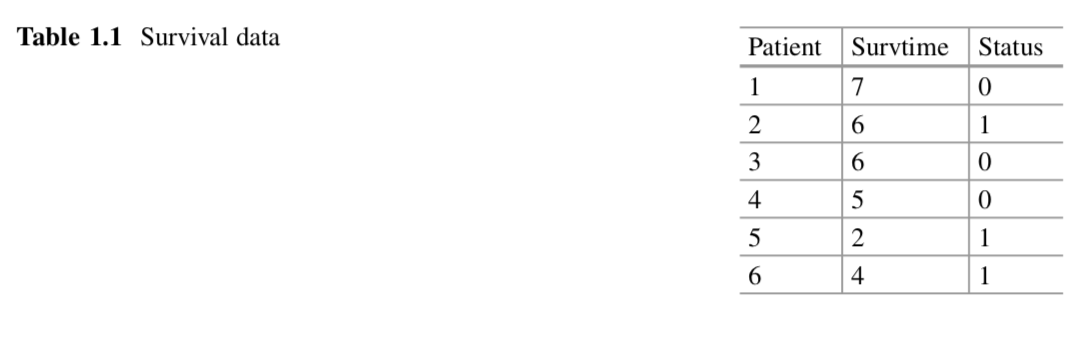
\includegraphics[scale = .35]{001.png}
	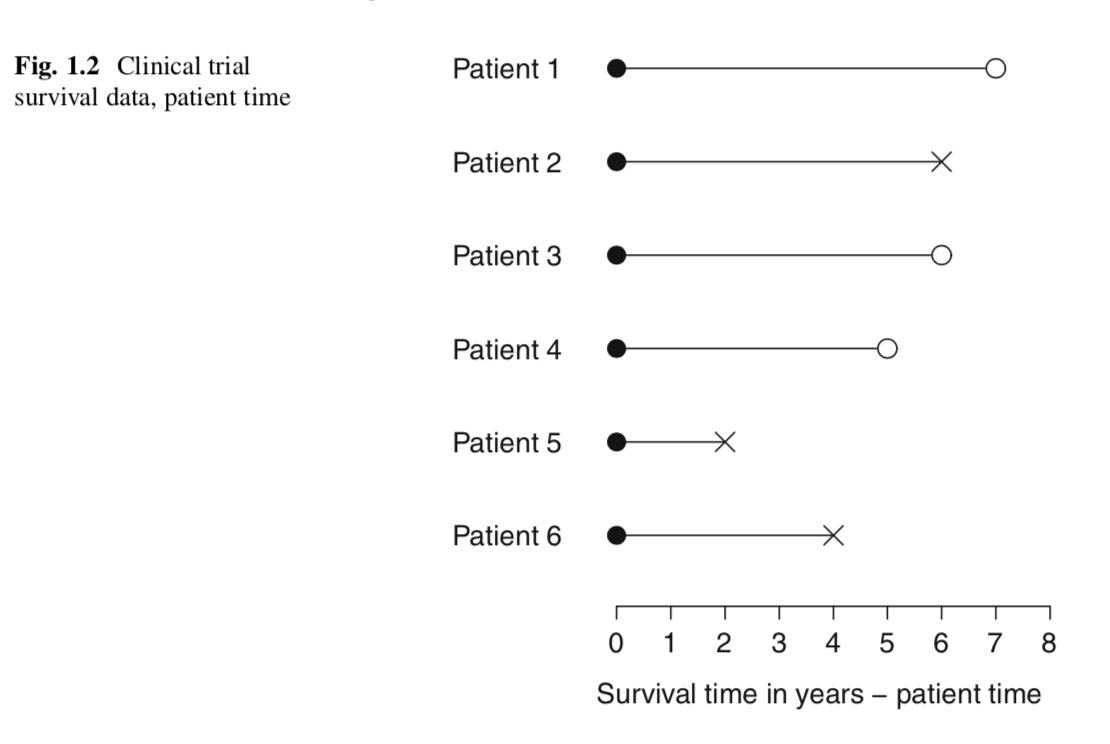
\includegraphics[scale = .35]{002.png}
\end{figure}
\begin{Verbatim}
> tt <- c(6, 7, 10, 15, 19, 25)
> delta <- c(1, 0, 1, 1, 0, 1)
> trt <- c(0, 0, 1, 0, 1, 1)
> survdiff(Surv(tt, delta) ~ trt)
[1]        N   Observed   Expected   (O-E)^2/E   (O-E)^2/V
trt=0      3      2         1.08       0.776       1.27
trt=1      3      2         2.92       0.288       1.27

Chisq= 1.3 on 1 degrees of freedom, p= 0.259
\end{Verbatim}
\begin{itemize}
\item Conclusion: The p-value is 0.259, indicating that the group difference is \empr{not statistically significant}.
\end{itemize}
\end{frame}

\section{Weighted log-rank test}
\begin{frame}
\frametitle{Weighted log-rank test}
\begin{defblock}{Cochran-Mantel-Haenzel Test}
A test for \empr{independence} of two factors (here, treatment and outcome) adjusted for a potential confounder(like log-rank test). 
\end{defblock}
\begin{itemize}
\item An important generalization of this test makes use of a series of $D$ {\color{red}weights $w_i$}, with which we may define a weighted log-rank test by:
\begin{itemize}
\item Mean: $U_0(w) = \sum w_i(d_{0i} - e_{0i})$
\item Variance: $var(U_0) = \sum {w_i}^2v_{0i} = V_0(w)$
\end{itemize}
\item The most common way of setting weights is:
\begin{itemize}
\item $w_i = \lbrace \hat{S}(t_i)\rbrace^{\rho}$
\item $\rho = 0$: log-rank test
\item $\rho = 1$: prentice modification
\end{itemize}
\item A log-rank test using these weights is called the {\color{red}Fleming-Harrington $G(\rho)$ test}.
\end{itemize}
\end{frame}

\pagebreak
\begin{frame}[fragile]
\frametitle{Example}
\begin{itemize}
\item The effect of this test is then to place \empr{higher weight} on {\color{red}earlier} survival differences.
\end{itemize}
\begin{Verbatim}
> head(pancreatic)
[1]   stage       onstudy      progression        death
1      MPC      12/16/2005       2/2/2006      10/19/2006 
2      MPC        1/6/2006      2/26/2006       4/19/2006
3      LAPC       2/3/2006       8/2/2006       1/19/2007
4      MPC       3/30/2006           <NA>       5/11/2006 
5      LAPC      4/27/2006      3/11/2007       5/29/2007 
6      MPC        5/7/2006      6/25/2006      10/11/2006
\end{Verbatim}
\begin{itemize}
\item Died with no recorded, shown ``\texttt{NA}'', so \pkg{PFS} is time to death, otherwise \pkg{PFS} is time to the date of progression.
\end{itemize}
\begin{Verbatim}
> attach(pancreatic)
> # convert the text dates into R dates
> Progression.d<-as.date(as.character(progression))
> OnStudy.d<-as.date(as.character(onstudy))
> Death.d<-as.date(as.character(death))
\end{Verbatim}
\end{frame}

\pagebreak
\begin{frame}[fragile]
\frametitle{Example by log-rank test}
\begin{Verbatim}
> #compute progression free survival
> progressionOnly<-Progression.d - OnStudy.d
> overallSurvival<-Death.d-OnStudy.d
> pfs<-progressionOnly
> pfs[is.na(pfs)]<-overallSurvival[is.na(pfs)]
> #convert pfs to months
> pfs.month<-pfs/30.5
> #note that no observations are censored
> #plot
> plot(survfit(Surv(pfs.month) ~ stage), xlab="Time in months", 
ylab="Survival probability", col=c("blue", "red"), lwd=2) 
> legend("topright", legend=c("Locally advanced", "Metastatic"),
col=c("blue","red") , lwd=2)
\end{Verbatim}
\begin{itemize}
\item 	{\color{red}The log-rank test} is when {\color{red}$\rho=0$}
\end{itemize}
\begin{Verbatim}
> survdiff(Surv(pfs) ~ stage, rho=0)
[1]           N   Observed   Expected   (O-E)^2/E   (O-E)^2/V
stage=LA      8       8         12.3       1.49       2.25
stage=M      33      33         28.7       0.64       2.25

Chisq= 2.2 on 1 degrees of freedom, p= 0.134
\end{Verbatim}
\end{frame}
\pagebreak
\begin{frame}
\frametitle{Example by log-rank test}
\begin{figure}[h!]
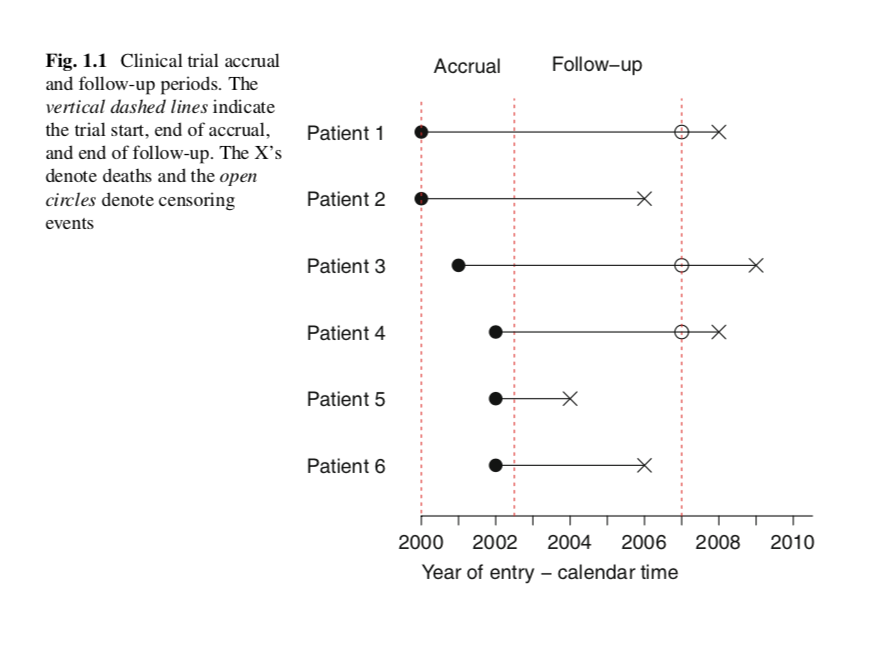
\includegraphics[scale = .4]{003.png}
\end{figure}
\begin{itemize}
	\item Conclusion: The p-value is 0.134, indicating that the \pkg{LA} and \pkg{M} difference is \empr{not statistically significant}.
\end{itemize}
\end{frame}

\pagebreak
\begin{frame}[fragile]
\frametitle{Example by Prentice modification}
\begin{Verbatim}
> survdiff(Surv(pfs) ~ stage, rho=1)
[1]           N   Observed      Expected   (O-E)^2/E   (O-E)^2/V
stage=LA      8      2.34          5.88       2.128       4.71
stage=M      33     18.76         15.22       0.822       4.71

Chisq= 4.7 on 1 degrees of freedom, p= 0.0299
\end{Verbatim}
\begin{itemize}
\item Conclusion: The p-value is 0.0299, indicating that the \pkg{LA} and \pkg{M} difference is \empr{ statistically significant}.
\item Explain:This version of the test places \empr{higher weight on earlier} survival times. From Fig last slide we see that indeed the \pkg{M} group shows an \empr{early survival advantage over} the locally advanced group, but the survival curves converge after about 10 months. The reason for the difference is that these two tests, with $\rho$ is 0 or 1, are optimized for different alternatives.
\end{itemize}
\end{frame}

\section{Stratified Tests}
\begin{frame}
\frametitle{Hypothesis Test}
\begin{itemize}
\item Compare two groups while adjusting for another \empr{covariate}, and if the covariate we are adjusting for is categorical with {\color{red}a small number of levels $G$}, we may construct a \empr{stratified log-rank test}.
\item Null hypothesis: $H_0: h_{0j}(t)=h_{1j}(t)$ for $j = 1,2,...,G$.
\item Each level of the second variable, compute a \empr{score statistic} $U_{0g}$ and variance $V_{0g}$, where $g = 1,2,...,G$ is the group indicator.
\item The test statistic is: 
${\chi}^2 = \frac{(\sum_{g=1}^{G}U_{0g})^2}{\sum_{g=1}^{G}{V_{0g}}^2}$
\item Compared to a $\chi _{1}^{2}$.
\end{itemize}
\end{frame}

\pagebreak
\begin{frame}[fragile]
\frametitle{Example by unstratified groups}
\begin{itemize}
\item \pkg{Treatment center}, \pkg{age group}, or \pkg{gender} are examples of variables need to stratify.
\item The primary goal is to compare the \empr{time to relapse} (defined in this study as return to smoking) between two treatment groups:
\end{itemize}
\begin{Verbatim}
> attach (pharmacoSmoking)
> survdiff(Surv(ttr, relapse) ~ grp)
[1]                N   Observed    Expected   (O-E)^2/E   (O-E)^2/V
grp=combination   61      37         49.9        3.36        8.03
grp=patchOnly     64      52         39.1        4.29        8.03

Chisq=8 on 1 degrees of freedom, p= 0.00461
\end{Verbatim}
\begin{itemize}
\item If we are concerned that the group comparison may differ by age, we may define a categorical variable
\end{itemize}
\begin{Verbatim}
> table(ageGroup2))
[1] ageGroup2
     21-49   50+
     66     59
\end{Verbatim}
\end{frame}

\pagebreak
\begin{frame}[fragile]
\frametitle{Example by stratified groups}
\begin{itemize}
\item The log-rank test stratified on ``\texttt{ageGroup2}'':
\end{itemize}
\begin{Verbatim}
> survdiff(Surv(ttr, relapse) ~ grp + strata(ageGroup2))
[1]                N   Observed    Expected   (O-E)^2/E   (O-E)^2/V
grp=combination   61      37         49.1        2.99        7.03
grp=patchOnly     64      52         39.9        3.68        7.03

Chisq=7 on 1 degrees of freedom, p= 0.008
\end{Verbatim}
\begin{itemize}
\item Conclusion: The chi-square test in this case \empr{differs only slightly} from the unadjusted value, indicating that it was not necessary to stratify on this variable.
\end{itemize}
\end{frame}

\pagebreak
\begin{frame}[fragile]
\frametitle{Simulated Dataset}
\begin{problock}{Clinical trial comparison}
Set up {\color{red}a simulated dataset} from a clinical trial comparing a standard therapy ({\color{red}control = 0}) to an experimental therapy ({\color{red}treated = 1}). Suppose that the survival times are {\color{red}exponentially distributed}, and that the disease is rapidly fatal, so that there is {\color{red}no censoring}. We also suppose that there is a {\color{red}confounding variable}, ``\texttt{genotype}'', which can either be {\color{red}wild type} (i.e. normal) or {\color{red}mutant}, the data will shown below:
\end{problock}
\begin{Verbatim}
> lambda.mutant.0 <- 0.03
> lambda.mutant.1 <- 0.03*0.55
> lambda.wt.0 <- 0.03*0.2
> lambda.wt.1 <- 0.03*0.2*0.55
\end{Verbatim}
\end{frame}

\pagebreak
\begin{frame}[fragile]
\frametitle{Simulated Dataset}
\begin{itemize}
\item (1) set a ``\texttt{seed}'' for the random variable generator, so that this example may be reproduced exactly.
\item (2) generate exponential random variables and string them together into the variable ``\texttt{ttAll}''.
\item (3) create the censoring variable ``\texttt{status}''.
\item (4) create the treatment variable ``\texttt{trt}'' and \texttt{genotype}, as follows:
\end{itemize}
\begin{Verbatim}
> set.seed(4321)

> tt.control.mutant <- rexp(25, rate=lambda.mutant.0)
> tt.treat.mutant <- rexp(125, rate=lambda.mutant.1)
> tt.control.wt <- rexp(125, rate=lambda.wt.0)
> tt.treat.wt <- rexp(25, rate=lambda.wt.1)
> ttAll <- c(tt.control.mutant, tt.treat.mutant,
 tt.control.wt, tt.treat.wt)
> status <- rep(1, length(ttAll))
> genotype <- c(rep("mutant", 150), rep("wt", 150))
> trt <- c(rep(0, 25), rep(1, 125), rep(0, 125), rep(1, 25))
\end{Verbatim}
\end{frame}

\pagebreak
\begin{frame}[fragile]
\frametitle{Simulated Dataset}
\begin{itemize}
\item The survival plots comparing the two treatments is shown below(left).
\item The log-rank test appears to confirm this with a very \empr{strong} p-value.
\end{itemize}
\begin{Verbatim}
> survdiff(Surv(ttAll, status) ~ trt))
[1]        N   Observed    Expected    (O-E)^2/E   (O-E)^2/V
trt=0     150     150         183         6.00        15.9
trt=1     150     150         117         9.41        15.9
   
Chisq=15.9 on 1 degrees of freedom, p= 6.66e-05
\end{Verbatim}
\begin{figure}[h!]
	\includegraphics[scale = .38]{004.png}
\end{figure}
\end{frame}

\pagebreak
\begin{frame}[fragile]
\frametitle{Simulated Dataset}
\begin{itemize}
\item But plot the survival curves comparing treatment to control separately for the mutant and wild type patients(right of the Figure last slide), we see that \empr{within each genotype} the {\color{red}treatment is actually superior to the control}.
\end{itemize}
\begin{Verbatim}
> survdiff(Surv(ttAll, status) ~ trt + strata(genotype))
[1]        N   Observed    Expected    (O-E)^2/E   (O-E)^2/V
trt=0     150     150         133         2.17        7.57
trt=1     150     150         167         1.73        7.57

Chisq=7.6 on 1 degrees of freedom, p= 0.00595
\end{Verbatim}
\begin{itemize}
\item Explain:
\begin{itemize}
\item The treatment improves survival compared to the control.
\item Patients carrying the wild type form of the gene have better survival than do patients carrying the mutation.
\item There are more mutation-carrying patients in the treatment group than in the control group, whereas the reverse is true for wild type patients.
\end{itemize}
\end{itemize}
\end{frame}
\end{document}